\section{Los fundamentos del sistema nervioso.}

El sistema nervioso es la máquina química más compleja conocida y por conocer. Todo estudio del mismo está condenado a constantes huecos teóricos y amplias fronteras, muchas en eterna penumbra. Esta condición nace de una complejidad organizativa y no una fundamental, pues los elementos individuales son en gran parte bien entendidos. Más allá de las limitaciones de la neurociencia como campo novel, el conocimiento sobre la percepción está limitado por cuestiones metafísicas. Aun después de que el lector haya aceptado su propia existencia se plantean ciertos dilemas: existen casos de pacientes que han sufrido lesiones cerebrales y muestran cambios en su comportamiento tales que se vuelven irreconocibles ante sus seres queridos. Intentar explicar tales fenómenos utilizando conceptos de alta abstracción como \enquote{personalidad} o \enquote{alma} es un interesante juego intelectual, pero también un pozo de respuestas contradictorias. Es por ello que a la hora de estudiar estos fenómenos no podemos sino limitarnos a encontrar patrones en aquéllo que podemos observar y escribir un gran \enquote{NO LO SABEMOS} en lo que lo rodea.

Lo que procede no va a ser simple, pero en esencia se resume en:

\begin{enumerate}
	\item El sistema nervioso está compuesto por células llamadas neuronas.
	\item Una neurona puede comunicarse con otra(s) por medio de señales unidireccionales.
	\item Cadenas y redes de neuronas establecen circuitos funcionales que pueden configurar desde comportamientos sencillos (como mover la pierna de forma refleja) hasta otros complejísimos (como el estado emocional).
\end{enumerate}

Alterar el comportamiento de grupos de neuronas de manera muy sutil puede provocar reacciones en cadena perceptibles a mayor escala. Esto es lo que ocurre al administrar una droga, y se verá más en detalle próximamente.

\subsection{Los bloques del sistema nervioso.}

A las puertas de la treintena de edad y buscando estabilidad financiera, Camilo Golgi comenzó a trabajar en un hospital para enfermos crónicos en Abbiategrasso. En la cocina de su alojamiento y con poco más que un microscopio y utensilios autofinanciados, montó un laboratorio al que regresaba tras cuidar de sus pacientes para continuar investigando acerca de un misterio que lo perseguía: el agente responsable de la comunicación nerviosa. Golgi desarrolló un método con el que logró teñir algunas células del sistema nervioso de un color negro. Este descubrimiento histológico tanteó la posibilidad del entendimiento de la mente, algo inimaginable en el siglo XIX. Irónicamente, su figura se vio eclipsada por la del científico español Santiago Ramón y Cajal que, utilizando su mismo método, construyó teorías mucho más acertadas que él.

Las células --- llamadas células nerviosas o neuronas --- tenían una estructura ramificada e interconectada que formaba amplias redes. Los dos científicos diferían en un sencillo detalle: ¿eran las neuronas células independientes como decía Cajal o actuaban como un tejido continuo sin separación interna como pensaba Golgi? Este enfrentamiento se cerró definitivamente con la invención del microscopio electrónico y el descubrimiento de una breve interrupción entre neurona y neurona: el espacio sináptico (Figura \ref{synapse}-C$_1$).

\begin{figure}[H]
	\centering

	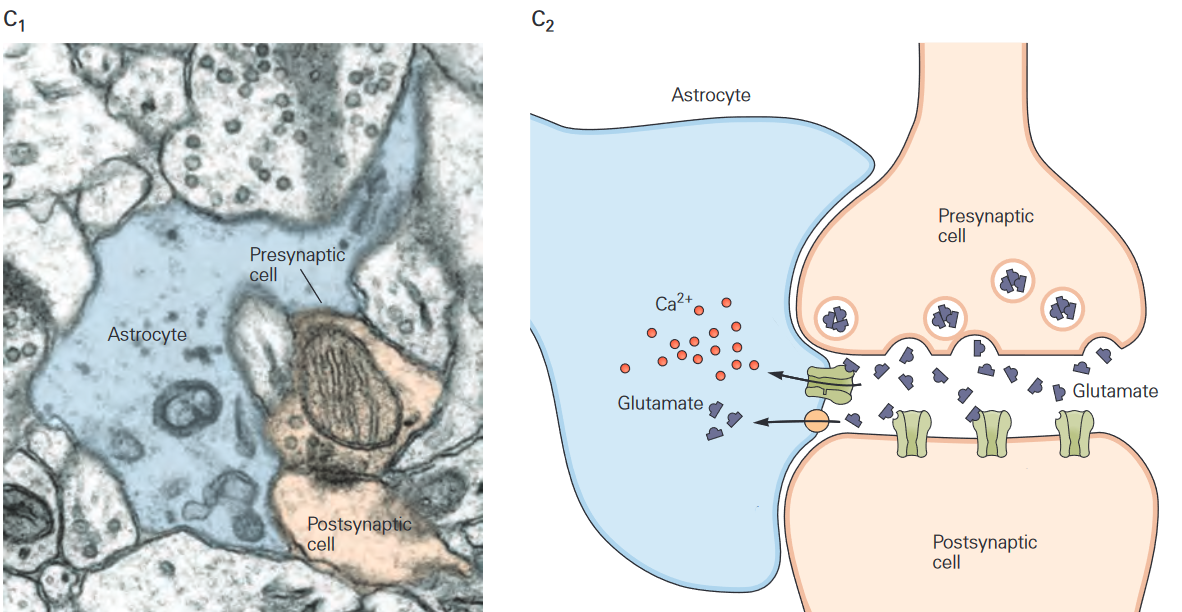
\includegraphics[width=\linewidth]{media/3-synapse.png}
	\caption{(C$_1$) Células del SN vistas bajo microscopio electrónico. En naranja, las neuronas separadas por el espacio sináptico. En azul, un astrocito encargado de suministrarlas. (C$_2$) Vista esquemática. Ante un potencial de acción se abren canales de calcio. El calcio desencadena la fusión de las vesículas sinápticas con la membrana celular (exocitosis), liberando neurotransmisores (glutamato) al espacio sináptico. Los neurotransmisores se unen a los receptores de la neurona postsináptica, pudiendo causar diversos efectos. Luego son recaptados por la neurona o por el astrocito.}
	\label{synapse}
\end{figure}

Este conflicto sin embargo era hijo de una guerra que se libraba desde tiempos de Descartes. La guerra entre quienes creían que el sistema nervioso actuaba como un todo y quienes pensaban que se dividía en partes funcionales localizadas. Subproductos de esta lucha fueron personas como Franz Joseph Gall que, partiendo de la localización de las partes, ideó la frenología: un método de estudio de la personalidad a través de la medición de la forma de la cabeza que posteriormente fue empleado por teóricos del racismo como justificación científica (Figura \ref{gall}). Esta idea se veía contrapuesta a opiniones como la de Pierre Fluorens que, poniendo a prueba las tesis de Gall, concluyó que todas las partes del cerebro se encargan de todas las operaciones mentales. Una reacción no solo científica sino cultural, pues la reducción del alma a la actividad interna de una red de órganos era algo inaceptable para el contexto europeo.

\begin{figure}[H]
	\centering

	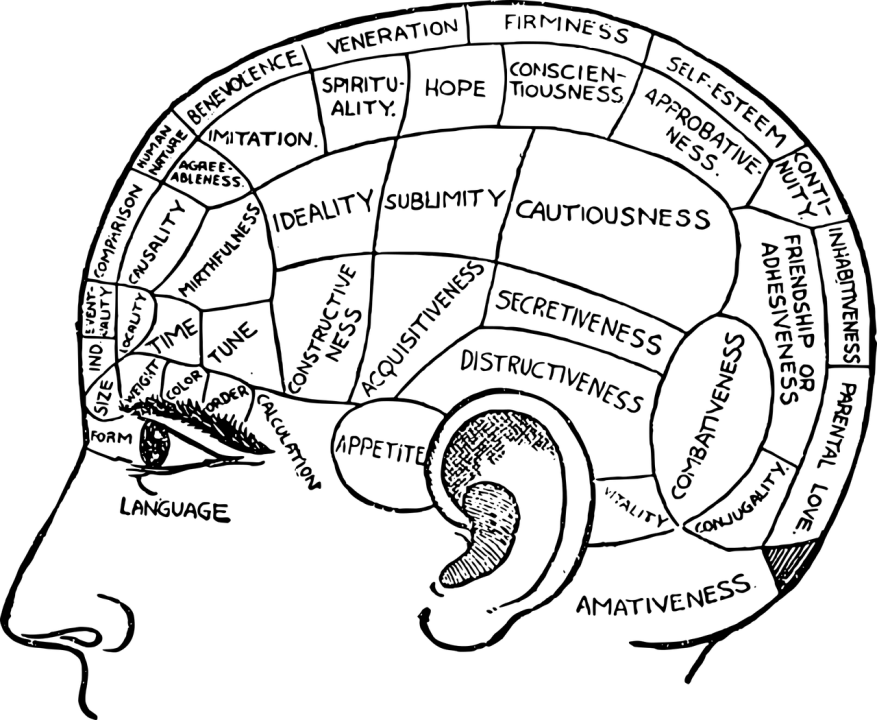
\includegraphics[width=\linewidth]{media/4-gall.png}
	\caption{Mapa funcional de la cabeza según Franz Joseph Gall. Sus métodos de asociación entre partes y funciones eran bastante pobres y sus teorías se vieron falsadas, pero la idea de utilizar medidas del cráneo como indicador de la personalidad fue utilizada como fundamento para las teorías racistas.}
	\label{gall}
\end{figure}

El pensamiento actual al respecto es algo mixto. Si bien se reconoce que tareas muy complejas como las emociones son desempeñadas en muchos circuitos distribuídos a lo largo de regiones variadas, también se acepta que estas se pueden descomponer en tareas más sencillas que generalmente sí son localizables.

\subsection{Estructura y organización.}

El entorno proporciona a los organismos un torrente continuo de información: radiación electromagnética, variaciones en la presión del aire, vibraciones en el suelo... Existen órganos con receptores capaces de reaccionar a estas variaciones en el medio: los órganos sensoriales. A las variaciones percibidas por un organismo a través de estos órganos se las denomina \textit{estímulos} (nótese que dependiendo del nivel de abstracción, un estímulo puede ser desde el tintineo de una campana hasta el impacto de un solo fotón). Cuando un órgano sensorial recibe un estímulo, este produce una señal sobre el sistema nervioso que generalmente concluye en la activación de otro órgano al que se denomina \textit{efector}. La acción realizada se denomina \textit{respuesta}, y si la respuesta es suficientemente compleja, la llamamos \textit{comportamiento}.

Entre el estímulo y la respuesta actúa el sistema nervioso: un conjunto de células que conducen señales eléctricas por distintas partes del organismo. Se divide en \textit{sistema nervioso central} (SNC), compuesto por el encéfalo y la médula espinal, y \textit{sistema nervioso periférico} (SNP), compuesto por todos los nervios que se ramifican del anterior. El SNP actúa como una autopista de información entre el SNC y los órganos sensoriales y efectores, mientras que el SNC se encarga de integrar y procesar los aportes del SNP para ofrecer una respuesta adecuada.

Por ejemplo, ante la presencia de una tarántula en la pierna (estímulo), los receptores sensoriales en la piel enviarán señales comunicando la información al SNC por medio de cadenas de neuronas (nervios) del SNP. En este momento y tras mirar a la tarántula, el SNC, configurado a lo largo de años por experiencias pasadas con arácnidos, concepciones culturales sobre las tarántulas o por simple predisposición genética podría activar a través del SNP músculos de la pierna para zarandearla y glándulas para segregar hormonas de estrés y miedo. El SNP entonces cuenta con dos vías: la \textit{aferente} (de los órganos sensoriales al SNC) y la \textit{eferente} (del SNC a los órganos efectores).

No todas las respuestas necesitan al encéfalo. Muchos comportamientos reflejos están autocontenidos en circuitos de la médula espinal. Sin embargo el encéfalo ofrece una capacidad de interpretación muy útil en seres vivos más complejos.

Las células del sistema nervioso que envían y reciben señales son las neuronas (Figura \ref{neuron}), pero en el sistema nervioso también hay otras células como la glía, que sirve de apoyo para las neuronas (Figura \ref{glia}). Desde la microglía con función inmunitaria hasta la macroglía, que recubre a las neuronas con una capa lipídica de mielina, las nutre controlando el paso de sustancias del torrente sanguíneo y controla las concentraciones de iones, neurotransmisores y elementos exógenos (Figura \ref{synapse}).

\begin{figure}[H]
	\centering

	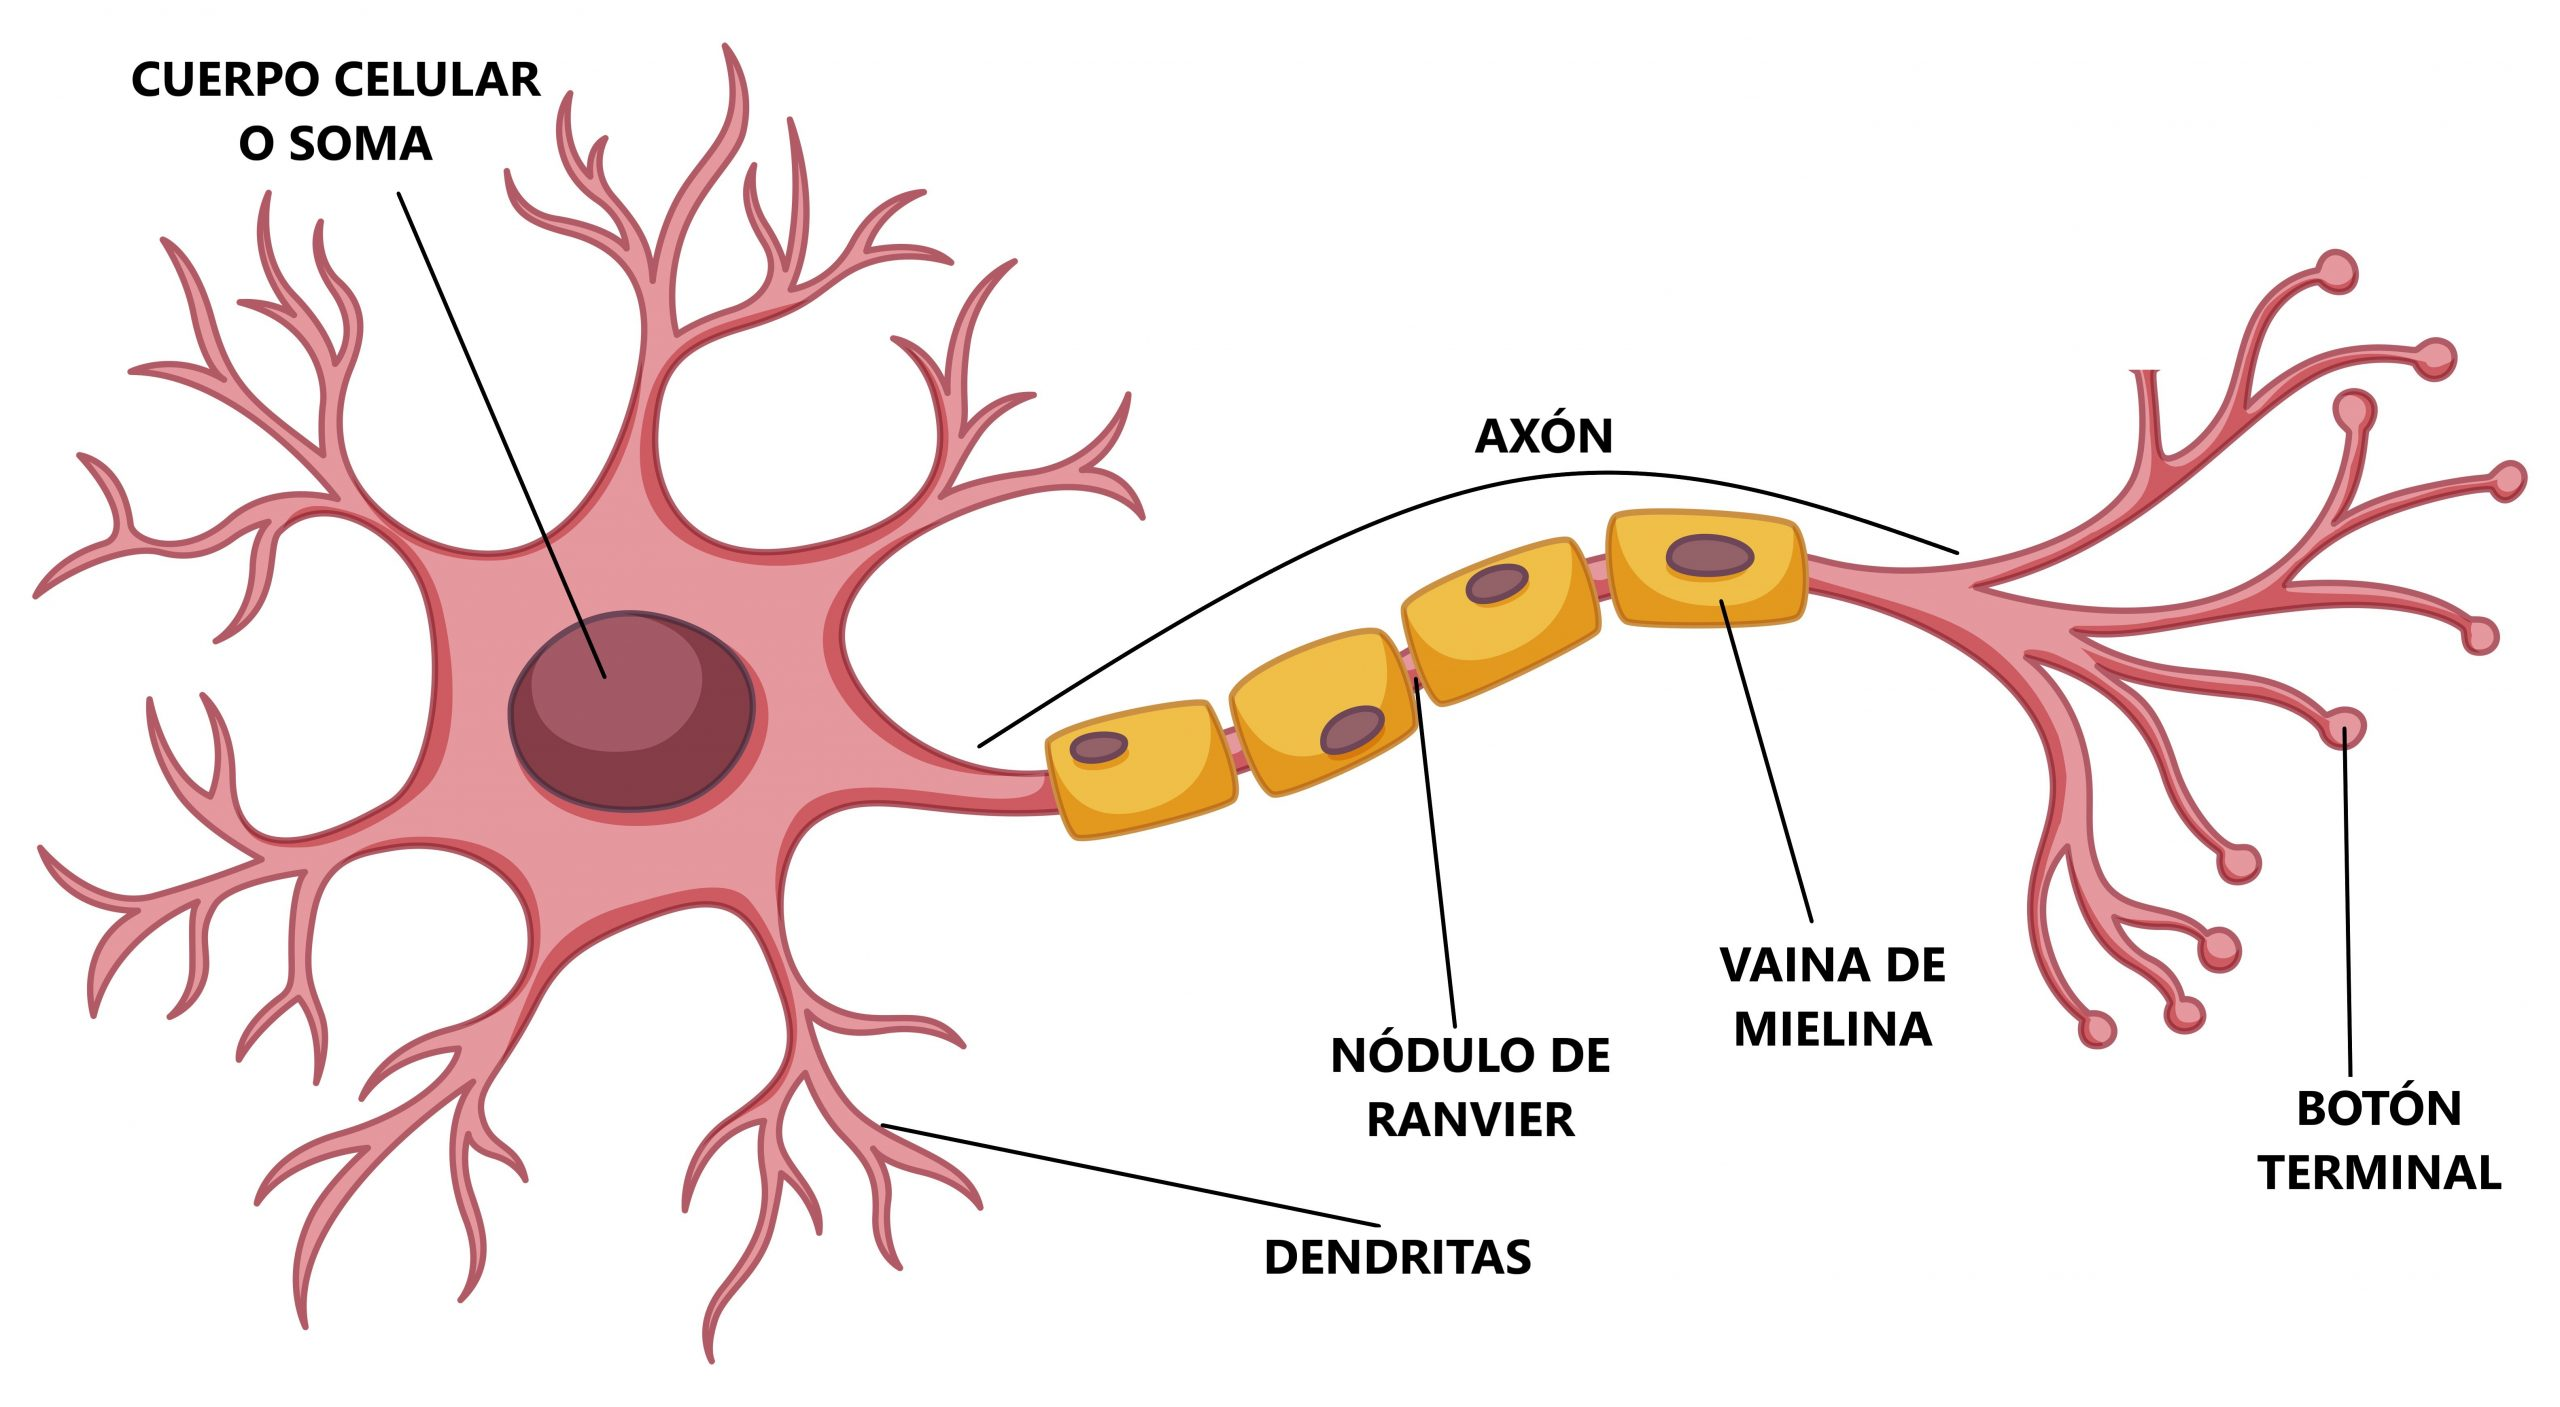
\includegraphics[width=\linewidth]{media/5-neuron.jpg}
	\caption{La neurona.}
	\label{neuron}
\end{figure}

\begin{figure}[H]
	\centering

	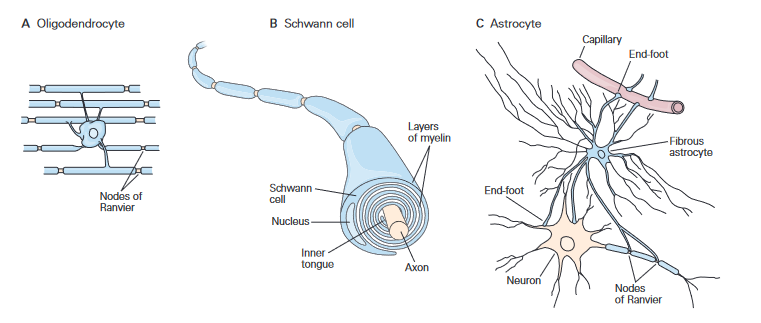
\includegraphics[width=\linewidth]{media/5-glia.png}
	\caption{Las células macrogliales.}
	\label{glia}
\end{figure}

\subsection{La neurona.}

Toda neurona está compuesta por tres partes: un soma o cuerpo celular, donde los procesos metabólicos habituales de toda célula ocurren; las dendritas, una estructura ramificada por la que entran las señales; y el axón, también ramificado y que envía señales a otras neuronas. El axón cumple una función integradora, pues en base a las diversas señales recibidas \enquote{decide} si disparar o no una señal hacia otras neuronas. Se denomina \textit{neurona presináptica} a aquélla que envía una señal, y \textit{neurona postsináptica} a aquélla que la recibe. Evidentemente estos son términos relativos, pues toda neurona es a la vez presináptica y postsináptica. ¿Cómo es posible la rapidísima comunicación que se observa en el sistema nervioso? Es necesario un análisis molecular.

En estado de reposo la neurona está polarizada, es decir, al igual que una pila, mantiene en todo momento una diferencia de potencial eléctrico entre su interior y su exterior de unos 70 milivoltios menos. Decimos que el interior está a -70 mV respecto del exterior. ¿De dónde nace este potencial y por qué no hay un cortocircuito instantáneo que lo calme? Todo depende de un delicado equilibrio (Figura \ref{action}).

Como toda célula, la neurona está delimitada por una bicapa fosfolipídica, por ende no permite el paso de sustancias cargadas como los iones. Al no permitir el paso de iones, es imposible el flujo de electricidad, por lo que el cortocircuito mencionado no sucede. Esta bicapa sin embargo se ve interrumpida por proteínas transmembranales llamadas \textit{canales}, cuya estructura forma un \enquote{túnel} por el que sí pueden circular iones. Estos canales son capaces de discriminar entre iones, dejando pasar a unos pero no a otros. Además, pueden abrirse y cerrarse bajo distintas condiciones, permitiendo o no el flujo.

Fuera de la célula, la concentración de iones de sodio (Na$^+$) es alta, mientras que dentro es baja. Por otra parte, la concentración de iones de potasio (K$^+$) fuera es baja, mientras que dentro es alta. Esta diferencia de concentración es mantenida por los riñones y la bomba de sodio-potasio, una proteína que introduce en la célula dos iones de K$^+$ por cada tres Na$^+$ que saca, consumiendo energía. Los iones entonces se ven expuestos a una fuerza electroquímica: la suma de la fuerza que intenta igualar el potencial en el exterior y el interior más la fuerza de difusión que intenta igualar las concentraciones internas y externas. Estas fuerzas producen un vaivén de iones que se desarrolla hasta alcanzar un equilibrio. El potencial interno durante este equilibrio se llama potencial de membrana.

En condiciones de reposo, los canales abiertos son más permeable a K$^+$ que a Na$^+$, por lo que, sumado a la acción de la bomba Na$^+$-K$^+$, el potencial de equilibrio es de -70 mV. Sin embargo, ciertas modificaciones fisicoquímicas pueden alterar esto. Por ejemplo, una entrada considerable de Na$^+$ puede llevar al interior de la célula a -55 mV (un potencial conocido como \textit{umbral}). En estas condiciones, los canales iónicos de Na$^+$ que se activan por voltaje se abren, desequilibrando el sistema y causando un flujo enorme de sodio. El nuevo potencial de equilibrio en estas condiciones es de unos +55 mV, y se conoce como \textit{potencial de acción}. El cierre de estos canales y la subsecuente acción de la bomba Na$^+$-K$^+$ recupera entonces el estado inicial del sistema hasta el siguiente desequilibrio.

\begin{figure}[H]
	\centering

	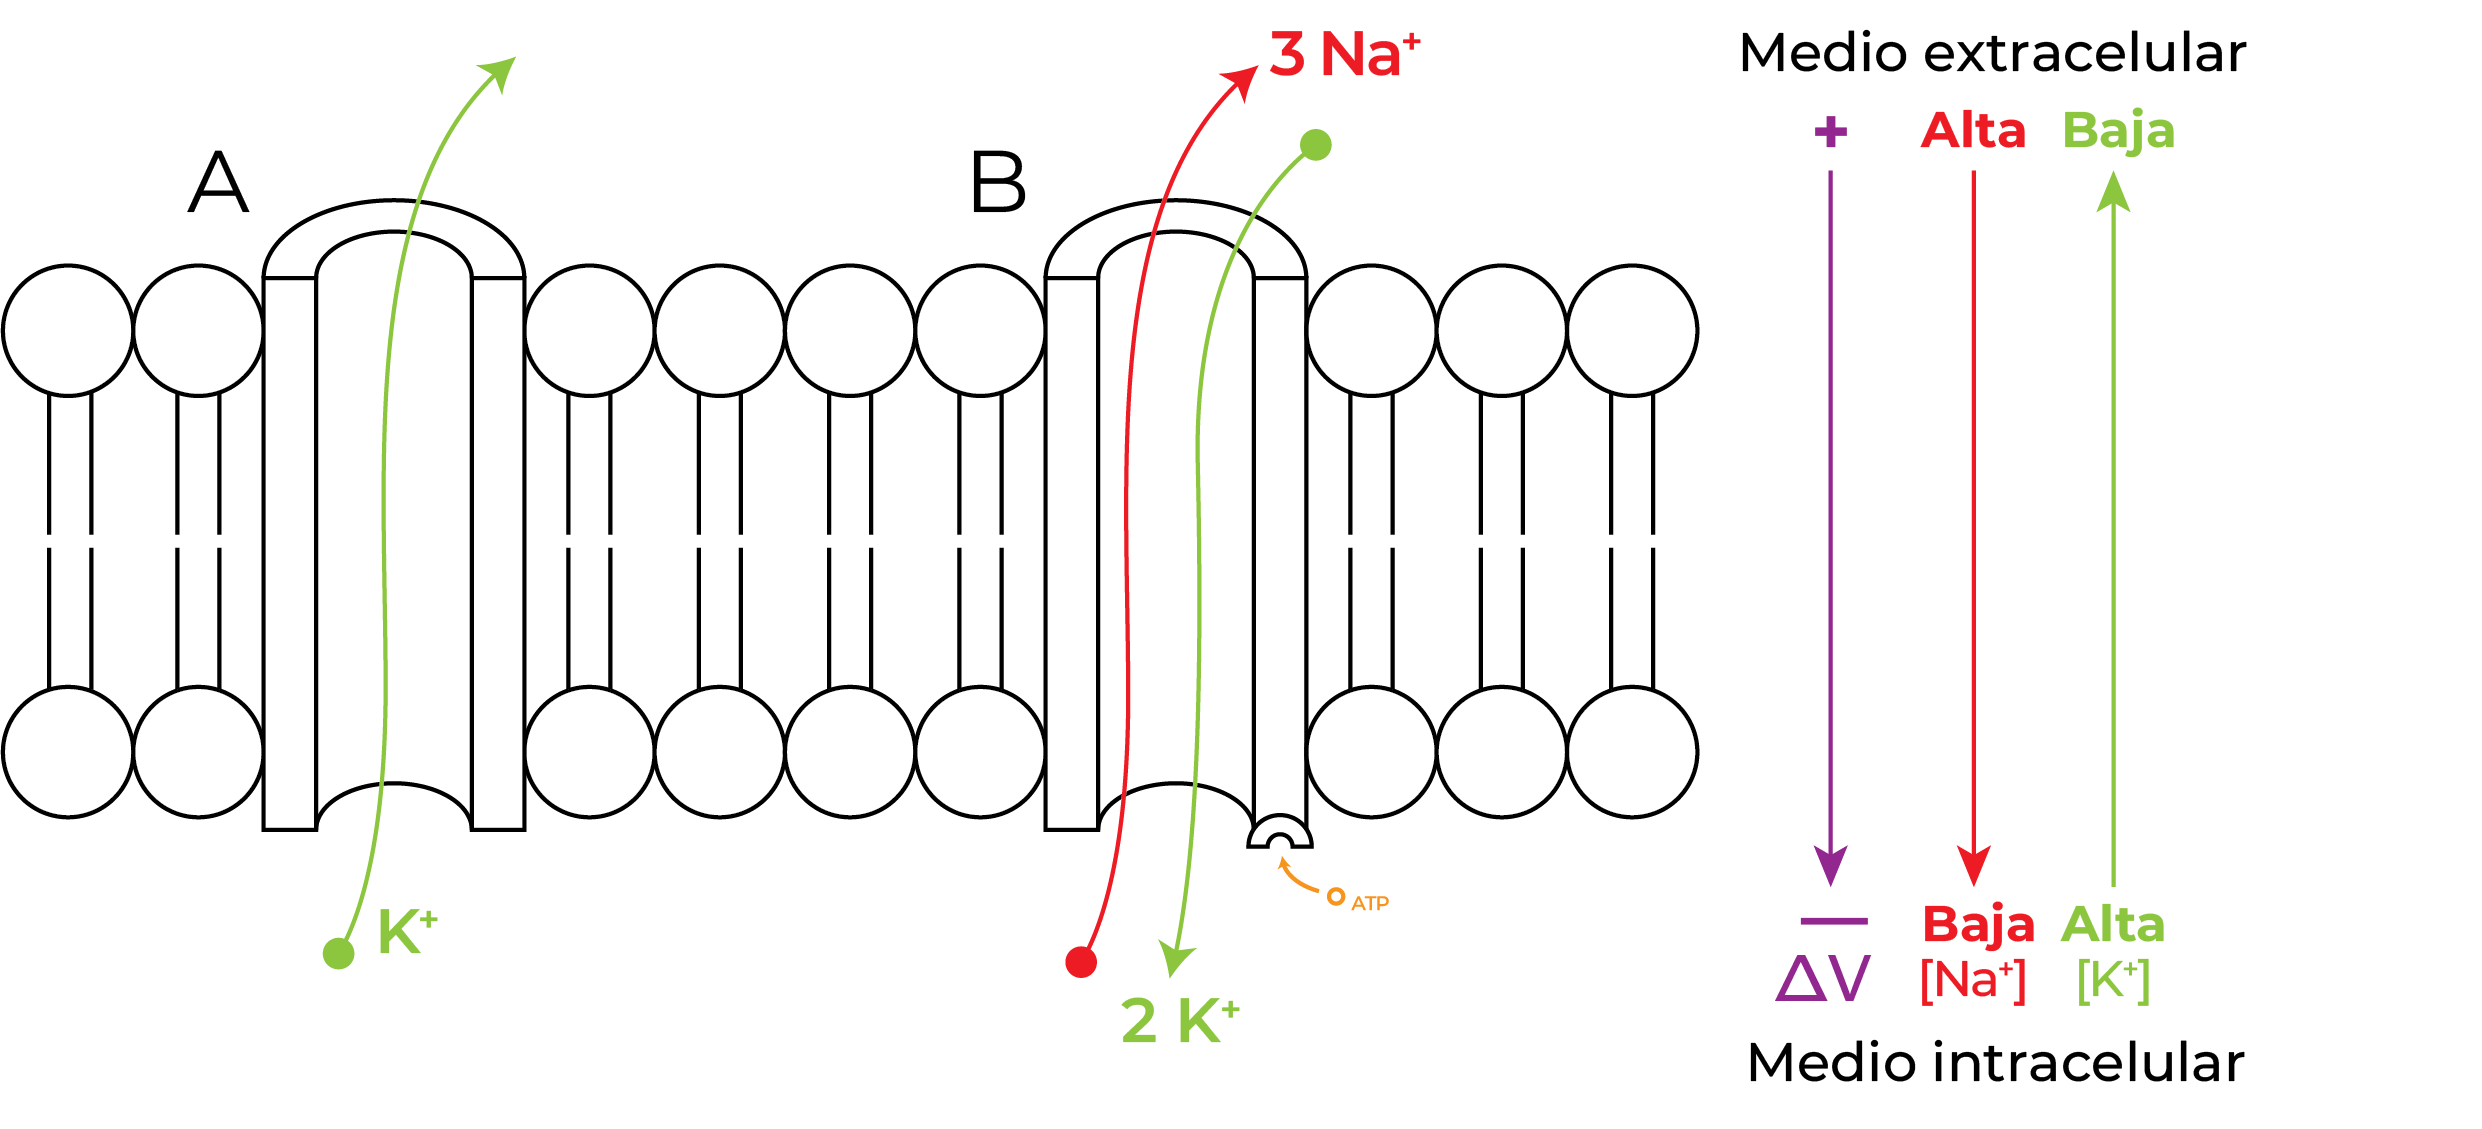
\includegraphics[width=\linewidth]{media/6-potencial.png}
	\caption{Vista transversal de la membrana celular. Contiene canales de potasio (A) y de sodio, que se abren principalmente durante el potencial de acción. La bomba de Na$^+$-K$^+$ (B) mantiene las concentraciones internas de estos iones.}
	\label{action}
\end{figure}

\begin{figure}[H]
	\centering

	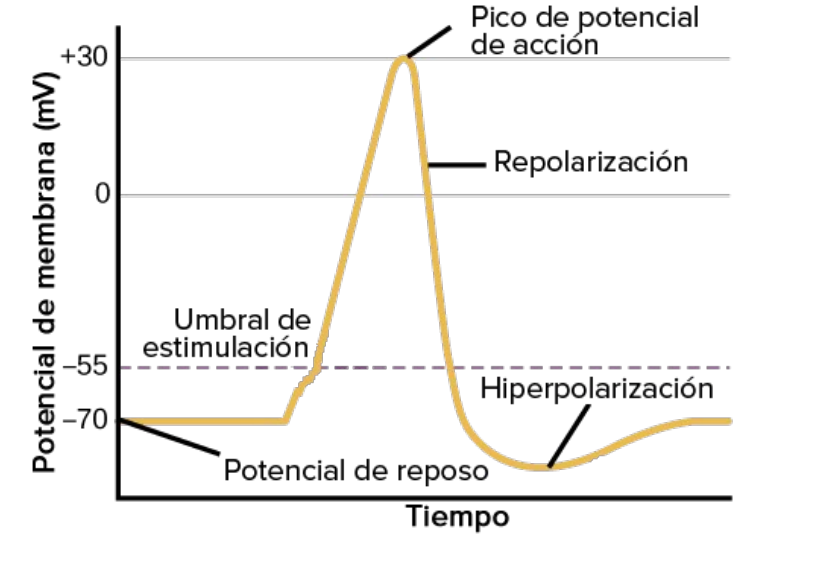
\includegraphics[width=\linewidth]{media/6-potencialgraph.png}
	\caption{Potencial de membrana a lo largo del tiempo.}
	\label{actiongraph}
\end{figure}

\subsection{Neurotransmisión.}

Los canales iónicos pueden abrirse y cerrarse debido a la unión de ciertas moléculas a las que denominamos \textit{neurotransmisores}. A cada receptor le corresponde un solo neurotransmisor. Los neurotransmisores son liberados por la neurona presináptica, que los almacena en pequeñas vesículas. Durante el potencial de acción se abren canales de Ca$^{2+}$. La entrada de calcio causa reacciones sobre las proteínas de las vesículas y la membrana celular que producen la fusión de ambas (exocitosis). Esta fusión, que puede ser total o parcial, libera los neurotransmisores contenidos en la vesícula hacia el espacio sináptico, donde viajan hasta llegar a los receptores de la neurona postsináptica a los cuales se unen. Las moléculas que se unen a receptores son denominadas \textit{ligandos} (Figura \ref{synapse}).

Al unirse a los receptores pueden hacer más o menos difícil que los canales se abran, sea directamente (en receptores ionotrópicos) o indirectamente produciendo cambios metabólicos en la célula (en receptores metabotrópicos). Si bien la acción depende del receptor y no tanto del transmisor, muchos neurotransmisores tienden a ser exclusivamente excitatorios (aumentan la probabilidad que se abran canales, aumentando también la de que se produzca una señal) o exclusivamente inhibitorios (disminuyen la probabilidad). Los aminoácidos glutamato y GABA por ejemplo son los principales encargados de la transmisión excitatoria e inhibitoria respectivamente.

Los neurotransmisores más importantes para nuestro caso son las catecolaminas (dopamina, norepinefrina y epinefrina), encargadas de funciones excitatorias, miedo, ira y recompensa; y la serotonina: crucial en la regulación del ánimo, la percepción y el sueño y muy relacionada con el LSD.

\subsection{Ejemplo: el reflejo rotular.}

El circuito neuronal que provoca el reflejo rotular es un ejemplo perfecto de lo expuesto hasta el momento. Estando la pierna flexionada, se percute el tendón de la rodilla. Su extensión causa un estrés sobre el cuádriceps femoral, lo cual provoca la activación de neuronas sensoriales, produciendo un impulso nervioso aferente excitatorio hasta la médula espinal. En la médula espinal se activan dos neuronas eferentes: una excitatoria hacia el cuádriceps femoral que libera acetilcolina sobre el músculo, un neurotransmisor responsable de su contracción; y una inhibitoria que evita la activación de la neurona análoga en el músculo complementario: el aductor (Figura \ref{sn}). De esta manera se coordina la contracción del cuádriceps con la no-contracción (y por ende extensión) del aductor, resultando en la extensión de la pierna. Las neuronas excitatorias se comunican utilizando el glutamato como neurotransmisor, las inhibitorias: GABA o glicina. La contracción del músculo es mediada por la liberación de acetilcolina sobre este.

\begin{figure}[H]
	\centering

	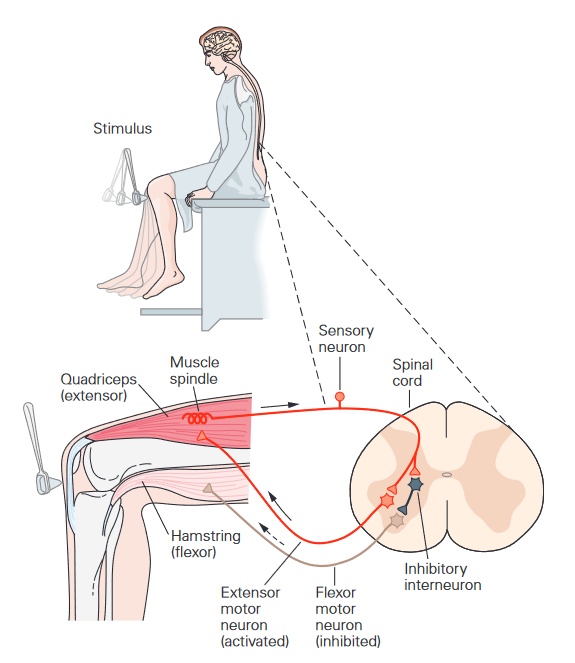
\includegraphics[width=.8\linewidth]{media/7-sn.png}
	\caption{El reflejo rotular.}
	\label{sn}
\end{figure}

Como abejas en un panal, las neuronas se agrupan en niveles de organización cada vez más complejos produciendo facultades como los sentidos y la memoria, construyendo los fenómenos emergentes que son el individuo y – quizás – la consciencia.

En estas tareas más complejas no solemos tratar con nervios ni neuronas individuales, sino que más bien observamos cómo se activan poblaciones de neuronas en regiones aproximadas del encéfalo. Estas regiones pueden interactuar unas con otras. A veces están asociadas anatómicamente, otras funcionalmente, y otras por el neurotransmisor que usan para comunicarse. Así, cuando una persona está feliz, quizás hay más actividad en tal o cual región, mientras que si está asustada, quizás las regiones que segregan este o aquél neurotransmisor se inhiben.

Lamentablemente es necesario dar cierto \enquote{salto de fe} para establecer una conexión entre psicología y neurobiología. Esto hace muy difícil tratar trastornos relacionados con la mente, pues al no comprenderse en su totalidad los fundamentos biológicos tras ellos, no es posible administrar una medicina infalible para curarlos. Este hueco de conocimiento permite la intrusión de chamanismos y vedismos, si bien en buena parte erradicados de su componente ritualístico-espiritual en la medicina moderna.

\newpage
